\chapter{Result Analysis}
In this section, we analyse the experiment results that we obtained and analyse the underlying reasons for the observation. We'll discuss the overall performance of all the methods that we applied and compare some particular methods with others. Also, we'll discuss how these algorithms would change as environment changes.
\section{Overall performance}
The performance of 10 methods that we used in the experiment various as a whole, even for a particular method, its performance may change for different query. However, the overall performance across 44 queries that we have assessed in the experiment of some methods show a superiority than others, while others cannot outperform others in most cases.We applied both binary and non-binary methods to give an image of how these algorithms performs and how they differentiate from each other. 

The binary evaluation method, precision at 10(prec@10) separate documents into two categories, relevant and irrelevant documents. In the experiment procedure, we developed a judgement platform following graded judgement principle, which resulted a list of document score that is non-binary. These score ranges from 0 to 4, from 0, which says the document is totally irrelevant to the topic to score 4, which means the document is comprehensively relevant to the topic. So a straightforward thinking is to regard documents score in the range from 1 to 4 as relevant documents and others as irrelevant documents. So then we get a distribution of the prec@10 of all methods running on all the 44 queries, as it is displayed in the Figure \ref{fig:prec10_dis} 
\begin{figure}
\centering
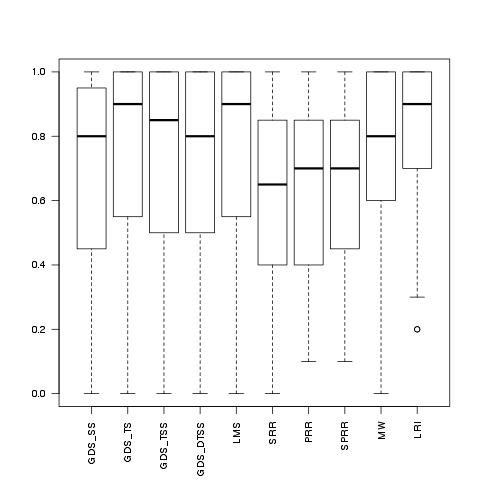
\includegraphics[scale=0.6]{images/prec10}
\caption{precision@10}
\label{fig:prec10_dis}
\end{figure}
The distribution of prec@10 demonstrates that of all these algorithms, there seems not be huge differences between other except the three round-robin methods show disadvantages over others. A obvious phenomenon that we can see from the figure is that mean precisions are all very high than a mean precision we can achieve in a traditional information retrieval system. The reason underlying these results is that different from a conventional search engine. The meta-search system conduct ranking based on the documents that are retrieved by their original search engines, so they are all originally retreated as relevant documents. So that means the overall proportion of relevant documents is larger than a traditional search engine. And also, the prec@10 only cares about the percentage of relevant documents among the top 10 retrieved documents, regardless of the degree of relevance and the rank of relevant documents. The little difference between methods make it tricky to find pattern inside these algorithms, especially a set of similar algorithms, we did a paired t-test to those algorithms to the same group, and we can see the results in Table \ref{tb:pvalue-gds} and Table \ref{tb:pvalue-RR}. As we can see from p-value, only the one paired of algorithms, namely GDS\_TS and LMS, rejected the Null Hypothesis, which means there is no sufficient confidence to say a algorithm is better than others.      

\begin{table}
\centering
\small
\begin{tabular}{lllll}
		&GDS\_SS&GDS\_TS&GDS\_TSS&LMS\\
		\cmidrule(lr){2-5}
GDS\_SS	&	-	&0.06315	&0.2001	&0.03484	\\
GDS\_TS	&		&	-	&0.1297	&0.5189	\\		
GDS\_TSS&		&		&	-	&0.08983	\\
LMS		&		&		&		&-\\
\end{tabular}
\footnotesize
\caption{p-value on t-test over GDS-XX methods and LMS, on confidence level of 95\%, freedom degree=43}
\label{tb:pvalue-gds}
\end{table}

\begin{table}
\centering
\small
\begin{tabular}{llll}
		&SRR&PRR&SPRR\\
		\cmidrule(lr){2-4}
SRR	&	-	&0.6748	&0.3071\\
PRR	&		&	-	&0.2528\\		
SPRR&		&		&	-\\
\end{tabular}
\footnotesize
\caption{p-value on t-test over Round-Robin methods and LMS, on confidence level of 95\%, freedom degree=43}
\label{tb:pvalue-RR}
\end{table}

We can also increase the standard of relevance, which means we restrict the criteria for relevant documents, and thus set the threshold of relevance, if we set threshold to 1, only the documents whose score and higher than 1 can be regarded as relevant documents and vice verse.

\begin{figure}[ht]
\centering
\subfigure[Threshold=1]{%
	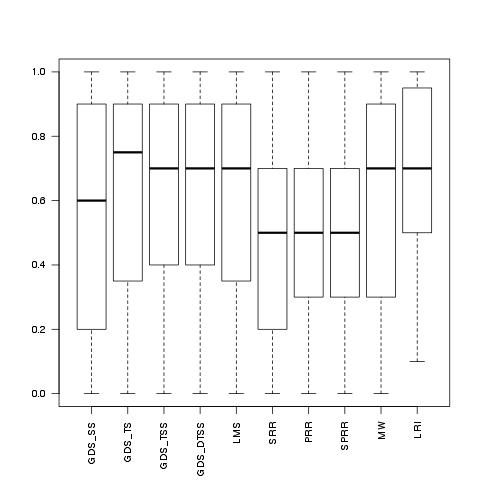
\includegraphics[scale=0.4]{images/prec10_1}
	\label{fig:prec10_1}
	}
\quad
\subfigure[Threshold=2]{%
	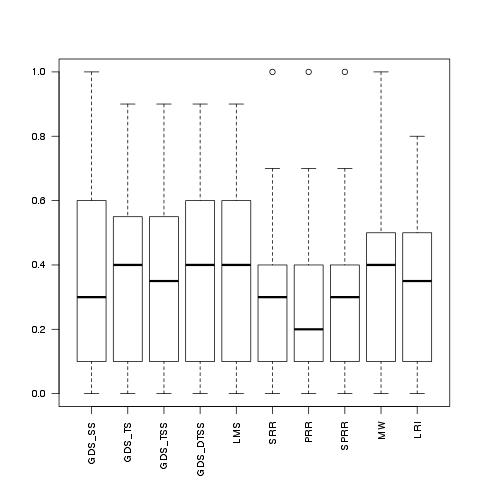
\includegraphics[scale=0.4]{images/prec10_2}
	\label{fig:prec10_2}
	}
\quad
\subfigure[Threshold=3]{%
	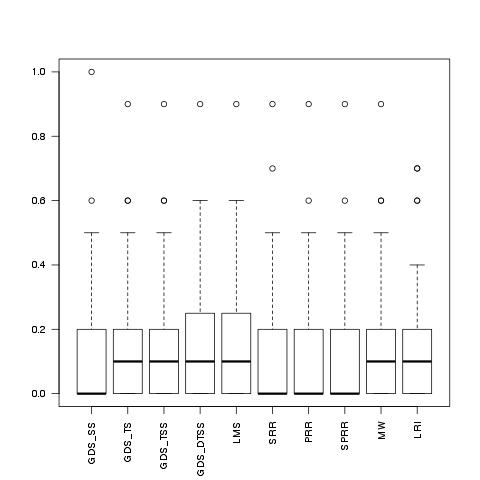
\includegraphics[scale=0.4]{images/prec10_3}
	\label{fig:prec10_3}
	}
\quad
\subfigure[Threshold=4]{%
	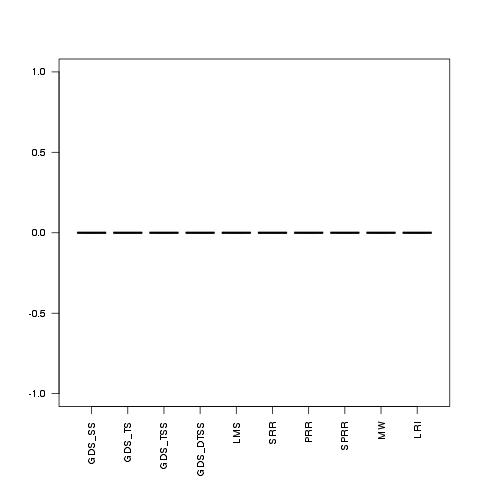
\includegraphics[scale=0.4]{images/prec10_4}
	\label{fig:prec10_4}
	}
\quad
\caption{Precision at different thresholds}
\label{fig:prec_mul}
\end{figure}

So the four graphics in Figure \ref{fig:prec_mul} illustrates the changes when we increase the threshold from 0 to 4. And one thing can be found is that the whole distribution of all methods has become lower as threshold is increases, however, the relatively distributions of algorithms against others are not significantly differentiates.

The other approach that we used to evaluate these different methods is a non-binary measurement method, NDCG@10, which calculate the gain score cumulatively. So ideally, NDCG@10 can reveal the differences between the resulted rank and the ideal rank according to the relevance scores assigned by the assessors.

\begin{figure}
\centering
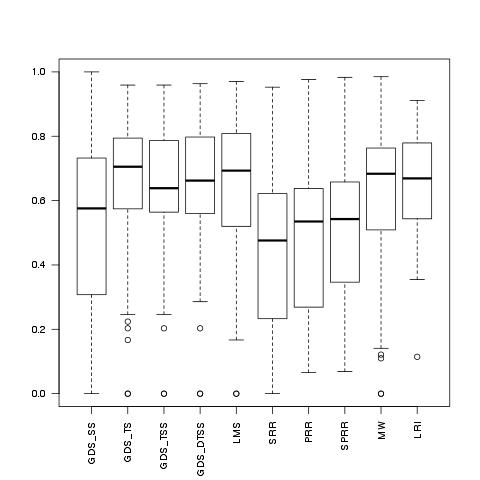
\includegraphics[scale=0.6]{images/ndcg@10}
\caption{NDCG@10 of all algorithms}
\label{fig:ndcg10_dis}
\end{figure} 

Figure \ref{fig:ndcg10_dis} is the distribution of the NDCG@10 score of all methods among all the 44 queries. Clearly, it makes a distinguishable distribution across different algorithms. Again we did a paired T-test on this algorithms, see Table \ref{tb:ttest-allndcg}

\begin{table}
\tiny
\begin{tabular}{p{1cm}p{1cm}p{1cm}p{1cm}p{1cm}p{1cm}p{1cm}p{1cm}p{1cm}p{1cm}p{1cm}}
&GDS\_TSS&GDS\_TS&GDS\_SS&GDS\_DTSS&LMS&SRR&PRR&SPRR&MW&LRI\\
\cmidrule(lr){2-11}
GDS\_TSS&---&NH&2.8873&NH&NH&4.7466&4.4734&3.7726&NH&NH\\

GDS\_TS&&---&3.2307&NH&NH&4.699&4.4148&3.8922&NH&NH\\

GDS\_SS&&&---&-3.0256&-3.1842&NH&NH&NH&NH&-3.4549\\

GDS\_DTSS&&&&---&NH&4.8382&4.5063&3.8844&NH&NH\\

LMS&&&&&---&4.7543&4.4829&3.9019&NH&NH\\

SRR&&&&&&---&NH&-3.51&-3.7406&-7.2133\\

PRR&&&&&&&---&-2.6575&-3.7114&-6.6232\\

SPRR&&&&&&&&---&-2.8994&-5.9037\\

MW&&&&&&&&&---&NH\\

LRI&&&&&&&&&&---
\end{tabular}
\footnotesize
\caption{T-test results for NDCG@10 results for all the methods,NH stands for Null Hypothesis, means t-test has not rejected the Null Hypothesis, the t test conducted from row to column, confidence level=95\%, df=43}
\label{tb:ttest-allndcg}
\end{table}
So now there exists significantly differences among different algorithms. The three Round Robin algorithms are the worst algorithms among all those algorithms been tested while the Local Re-index method and the Generic Document Scoring method based on Document Title (GDS\_TS) seems to be two outstanding algorithms among others in this environment. 
{\color{red} how to use table \ref{tb:effect size}}
\begin{table}
\tiny
\begin{tabular}{p{1.2cm}p{1.2cm}p{1.2cm}p{1.2cm}p{1.2cm}p{1.2cm}p{1.2cm}p{1.2cm}p{1.2cm}p{1.2cm}p{1.2cm}}
&GDS\_TSS&GDS\_TS&GDS\_SS&GDS\_DTSS&LMS&SRR&PRR&SPRR&MW&LRI\\
\cmidrule(lr){2-11}
GDS\_TSS&---&p=0.2849241, d=0.164888&p=0.2849241, d=0.164888&p=0.6570079, d=0.3138873&p=0.3382643, d=0.1880336&p=2.310635e-05, d=-0.3719031& p=5.558954e-05, d=-0.3399154&p=0.0004892817, d=-0.2528957&p=0.1742379, d=0.1083292&p=0.4817434, d=0.2449329\\
GDS\_TS&&---&p=0.00236984, d=-0.1806192&p=0.3820464, d=0.2059694&p=0.9073363, d=0.4548726&p=2.695421e-05, d=-0.3664063&p=6.6984e-05, d=-0.3329079&p=0.0003407972, d=-0.2682688&p=0.1011739, d=0.05668385&p=0.718813, d=0.3407105\\
GDS\_SS&&&---&p=0.004178282, d=-0.1519879&p=0.002699161, d=-0.1741874&p=0.1019622, d=0.05733364&p=0.2573317, d=0.1521309&p=0.6824074, d=0.3246332&p=0.07800444, d=0.03465159&p=0.001250152, d=-0.2110751\\
GDS\_DTSS&&&&---&p=0.4223028, d=0.2219145&p=1.716752e-05, d=-0.3824303&p=5.005215e-05, d=-0.3438145&p=0.0003489795, d=-0.267274&p=0.1188498, d=0.07107689&p=0.5209916, d=0.2600118\\
LMS&&&&&---&p=2.254158e-05, d=-0.372781&p=5.393764e-05, d=-0.3410388&p=0.0003309153, d=-0.2695003&p=0.09512011, d=0.05130356&p=0.731365, d=0.3464438\\
SRR&&&&&&---&p=0.1272298, d=0.077384&p=0.001065238, d=-0.2184404&p=0.0005385612, d=-0.2487635&p=6.327192e-09, d=-0.6193184\\
PRR&&&&&&&---&p=0.01100594, d=-0.09882246&p=0.000587745, d=-0.2449703&p=4.531094e-08, d=-0.5663733\\
SPRR&&&&&&&&---&p=0.005865978, d=-0.1340298&p=5.046627e-07, d=-0.4967929\\
MW&&&&&&&&&---&p=0.1560281, d=0.09709265\\
LRI&&&&&&&&&&---\\
\end{tabular}
\caption{effect size}
\label{tb:effect size}
\end{table}

The LRI (Local Re-index) method fetch the original web pages that were retrieved and  treat them as a document collection. The method then use an traditional indexing approach on the document collection as what we usually do in a centralised indexing information system. The documents were then ranked based on the scores that were calculated by the similarity between the query and the document text. So the performance of LRI methods is totally depended on the performance of the indexing method as well as the accuracy of the scoring method. If a distributed information retrieved system is no worse than an index centralised information retrieval system, it is considered as an acceptable method.	So the LRI is regarded as baseline method for all other methods as a top performance regardless of its efficiency in the aspect of time and space. It is also quite obvious that the LRI methods outperforms others in most of the cases as we can see in both precison@10 and NDCG@10.

We use a pure round-robin method in the experiment and two other prioritized round-robin methods to give different to different collections to rank documents in an order of collection importance. The figures shown that the overall performance of all the round-robin method performs the worst among all other algorithms.
      
\section{Round-Robin}

Round-robin was the most fundamental mechanical that has been widely used in the early meta-search system. As it has been stated, round-robin method is based on the hypothesis that documents are distributed evenly in different collections, which means that if all the collections have an equally distribution of documents according to their relevance to the query, the method can gain an excellent result. However, due to the fact that the collection may have different weights on a particular topic in reality, and the situation when documents are evenly distributed in collections seldom happens. As a result, round-robin method can not outperform others in most cases, and since the rank of documents in each cycle is random, the performance of the methods various in different runs. We run the round-robin algorithm five times and compare them with the LRI method as well as two other prioritized round-robin methods. Also, to test the optimized performance of round-robin, we designed an optimized round-robin method(\textit{OPRR}), which use the final relevance score judged by assessors as a criteria of collection weight and run a collection weight based prioritized round-robin. The results are displayed in Figure \ref{fig:rr}.
\begin{figure}
\begin{center}
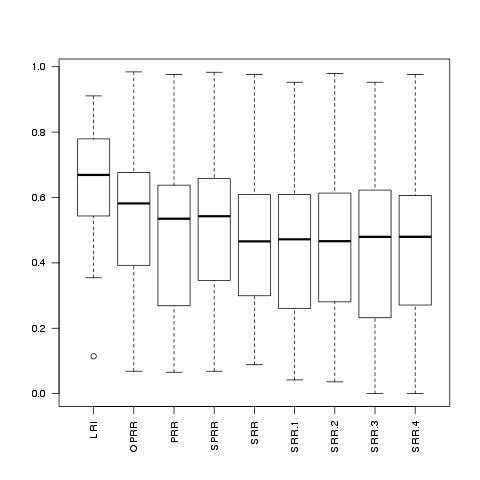
\includegraphics[scale=0.6]{images/RR_NDCG}
\label{fig:rr}
\caption{NDCG@10 of Simple Round Robin on 5 runs}
\end{center}
\end{figure}
As been stated, round-robin performs quite randomly in each run. The underlying reason is that documents were ranking  randomly in round-robin cycle. But, however, a phenomenon that we can observe from the Figure \ref{fig:rr} is that although these round-robin runs perform differently, the variation is not significant. The reason is because that we documents that lying in the top 10 list are pretty much the same in each run, and in that case, the difference is the relative order of these documents.    

Two other prioritized round-robin methods are also evaluated in the experiments. The original intention of both two algorithms is to rank collections in an order of relevance at the first place and then rank document in order of the collection score in each round-robin cycle. The PPR use the document length, namely the number of document retrieved, as an indication of collection relevance. The second prioritized round-robin method get the collection weight using the average similarity of the retrieved documents. This method is similar to a previous algorithm named \textit{TopSRR}\cite{Lu2005}, which use title and summary fields of top k documents to calculate the collection score. The original TopSSR method initialized two vectors $TV_j$ and $SV_j$ by merging all the title and summary fields together respectively and then use Equation to get the collection score.
\begin{equation}
S_j=c*Similarity(Q,TV_j)+(1-c)*(Q,SV_j)
\end{equation}   
In our method, we applied an average function on the similarity of all the top k documents that is retrieved. We then use the aggregated document similarity as the collection score in the round-robin method. As we can observe from Figure \ref{fg:ndcg10_dis}, both two algorithms have promote the median of NDCG@10 to some degree and make it more stable. We get a mean NDCG@10 by average the NDCG@10 of a query across all methods. Of all the 44 queries, the PRR method can perform better than mean NDCG@10 in 10 queries while SPRR can do better in 13 queries. That may suggest SPRR may get a more reasonable collection score than PRR.

\begin{figure}
\begin{center}
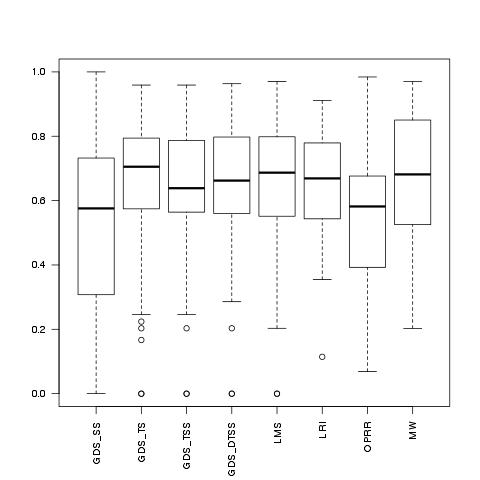
\includegraphics[scale=0.6]{images/OPRR}
\caption{NDCG@10 of OPRR with respect to other algorithms}
\label{fig:oprr}
\end{center}
\end{figure} 
The paired T-test (Table \ref{tb:tvalue-oprr})suggest that there exists distinguishable difference between the optimized round-robin. So that means neither of the two prioritized round-robin methods are sufficient to be optimized, and that remains a problem of collection weight, we'll discuss the topic in the next section.
 
\begin{table}
\centering
\small
\begin{tabular}{lll}
		&PRR&SPRR\\
\hline
OPRR	&5.0855&2.9621	\\
\end{tabular}
\footnotesize
\caption{t-value of t-test over OPRR to other prioritized Round-Robin, on confidence level of 95\%, freedom degree=43}
\label{tb:tvalue-oprr}
\end{table}
Even if we optimized the round-robin by providing an ideal collection score, the method is still not comparable to most of other merging algorithms, as shown in Figure \ref{fig:oprr}. The reason is round-robin methods itself is not a suitable method, which rank documents from different collections evenly  in a result. Saying we have 10 collections, one of which contains many relevant documents that would be ranked at top 10 in an ideal ranking and none of the remaining collections contain relevant documents. Using a round-robin method, even we rank the first document of the most relevant collection at the top of the final rank, all the other remaining nine documents in the list are irrelevant. As a result, the accuracy of the documents ranking compared to the ideal ranking is quite low.


\section{Evidence of Collection Weight}

Collection weight is always taken into consideration when doing a meta-search engine. The collection weight reveals the significance of a collection with respect to a topic. In an uncooperative environment, there exists limited information on the collection. So what the algorithms performance if we got an ideal or so called optimized collection score. We design a method that get the collection score by cumulate the relevance score that is assessed by assessors. And then we combined the score with the GDS\_DTSS method, we name it OGDS, means the optimized GDS. Figure \ref{fig:ogds} illustrates the importance of collection score, if we can add an ideal collection score to the algorithm, it can be improved in a large scale. The OGDS method, has improved the performance of the original GDS and even better than the LRI method. We examine how much difference from the weighted algorithms to the original by applying a Paired T-test(Table \ref{tb:odstt}). 

\begin{figure}
\begin{center}
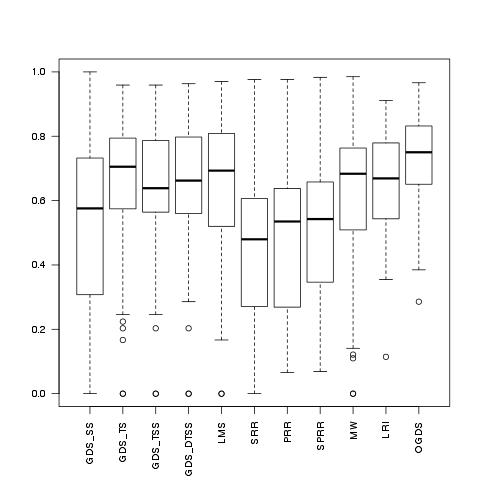
\includegraphics[scale=0.6]{images/OGDS}
\caption{NDCG@10 of OGDS with respect to other algorithms}
\label{fig:ogds}
\end{center}
\end{figure}
\begin{table}[h]
\caption{T-test result for SGDS}
\label{tb:odstt}
\centering
\begin{tabular}{lllllll}
\hline
  & GDS\_DTSS&GDS\_TS &GDS\_SS& LMS  & LRI     \\
\hline
 OGDS&4.4879 &3.6568&5.6473& 3.4213 & 2.966 \\ 
\end{tabular}
\caption{t-value of NDCG@10 of OGDS tested to other algorithms, confidence level 95\%, df=43}
\end{table}

\subsection{Document Length}

In our experiments, the limited information can be obtained from the result page. Number of documents retrieved from the search engine is usually accessible in the result page. In LMS, the document length, has been considered as the factor that represent the collection weight. We combined the collection weight get by the LMS with other score based algorithms, here we used the GDS\_DTSS method. As we can see from Figure \ref{fig:ndcg10_dis}, the LMS has increased the median of all the NDCG@10 across all the queries. But the total distribution has not been changed so much. Also, in the last section, we used LMS to get a collection weight in the prioritized algorithm PRR, and get the conclusion that LMS method cannot guarantee the optimized round-robin. Again, we used the method in previous section to get an optimized collection weight and combine it with the GDS\_DTSS, and compare it with the LMS algorithm. 


The LMS is much less than optimized as it is shown in the t-test in the round-robin experiment. The sizes of document collections themselves are various from each other in certain degree, so the number of documents retrieved by these collections are also influenced by the total number of documents as well as the precision of those search engines. For example, some search engines with a bad retrieval algorithm may return many inaccurate and irrelevant documents while some other search engines with high precision return a limited number of documents that is very relevant to the topic. So document length would not be a sufficient evidence of collection significance.

\subsection{Average document similarity}
Another method of getting the collection is by average the similarity of the text fields of all documents in the first result page with the topic. These text fields, in some way, is a sample of the document collection, which can reveal some information on the particular collection. 
 \begin{figure}
\begin{center}
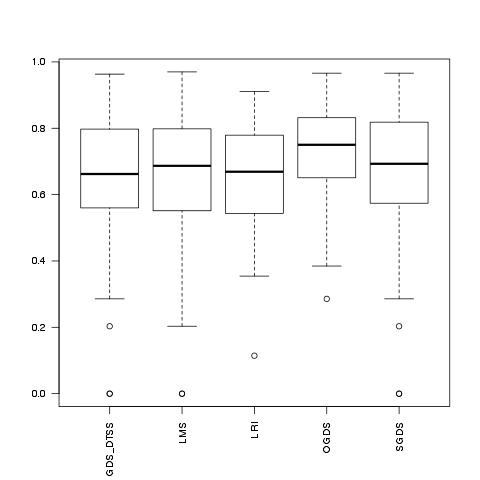
\includegraphics[scale=0.6]{images/SGDS}
\caption{NDCG@10 of SGDS with respect to other algorithms}
\label{fig:sgds}
\end{center}
\end{figure}



Compared to the document length based collection scoring method, LMS, the performance of average document similarity method is more close to the optimized collection weight.
\section{Value of document fields}
The GDS algorithms estimate the document collection score by a general scoring function using the text field provided by the result page. We used two fields, title and summary in our experiment, as text fields. We used four methods to estimate the document score, 

\begin{itemize}
\item
\textbf{GDS\_TS} Scoring function uses the title field only.
\item
\textbf{GDS\_SS} Scoring function uses the summary field only
\item
\textbf{GDS\_TSS} Scoring function uses the title field as the first priority, if score is not usable, use the summary field
\item
\textbf{GDS\_DTTS} Scoring function uses a combination of title field as well as summary field
\end{itemize}

The performance described by Figure \ref{fig:ndcg10_dis} shows that $GDS_SS$ performs the worst among all other general scoring functions, while $GDS\_TS$ performs the best. The phenomenon demonstrates the fact that the title may be more valuable than summary in representing the main topic of a document. Of all the 44 queries that we evaluated, $GDS_SS$ method can perform better than an average performance in 16 queries while $GDS\_TS$ can outperform others in most of the queries, making 33 of all.

\section{Parameter setting of multi-weight method}
To this point, we have taken four factors into our algorithms to get the final comparable document scores to rank the documents. The final method is named multi-weight because we took all these factors into consideration when calculating the document score. As we described in the experiment section, we set 4 weights to these four factors respectively and summarize the weighted factors. We test the performance of this method by a 4-fold cross validation.  

\begin{figure}
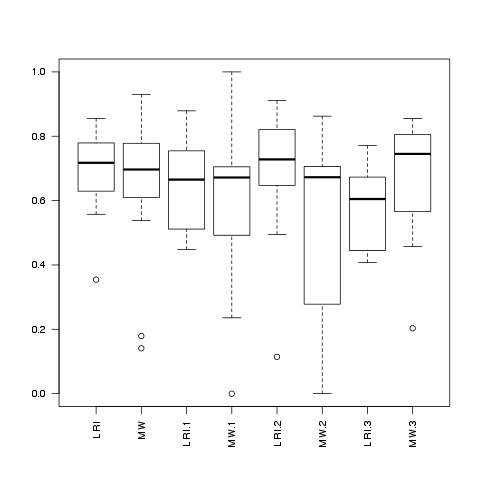
\includegraphics[scale=0.6]{images/4-fold}
\caption{4-fold cross validation}
\label{fig:4-fold}
\end{figure}

Figure \ref{fig:4-fold} is a result graphic of 4-fold cross validation compared with the LRI method. Each fold contains an equal number of randomly picked queries. As we can see the method varies among different folds. Sometimes it can outperform LRI in a great degree, for example, MW.3 with respect to the LRI method. However, it can perform very badly, for example, in MW.2. The purpose of the model is to set weights for those factors, so in a real world system, is the data size too small to learn?

